\begin{tikzpicture}[remember picture, overlay]
  \draw[line width = 4pt] ($(current page.north west) + (0.7in,-0.7in)$) rectangle ($(current page.south east) + (-0.7in,0.7in)$);
\end{tikzpicture}

\thispagestyle{empty}
\begin{center}
  \Huge \textbf{Supreme Court Statpack} \\
  \LARGE \textbf{October Term 2024-2025} \\
  \Large \textbf{(Extended Version)} \\ [7mm]
 % 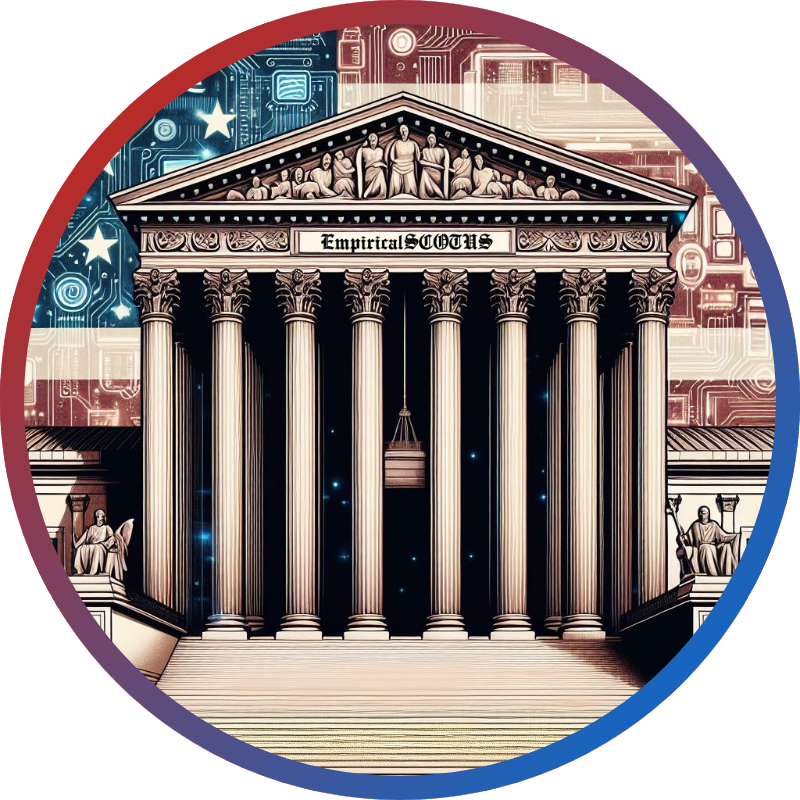
\includegraphics[width=300px]{images/empirical_scotus_logo.png}\\[2mm]
  %\textbf{EmpiricalSCOTUS} \\
  %\textit{Viewing the Supreme Court in an Entirely New Light} \\[3mm]
  \Huge \textbf{Need Direction Re: Logo} \\[3mm]

  \normalsize
  Compiled by Adam Feldman (J.D., Ph.D.) and Jake S. Truscott (Ph.D.) \\
  \vfill

  \footnotesize
  Version: 0.0 (Released) \\[2mm]

  \normalsize
 For additional data and accompanying analysis, please visit\\ \textcolor{blue}{\href{https://empiricalscotus.com/}{EmpiricalSCOTUS}} or \textcolor{blue}{\href{mailto:adam@feldmannet.com}{Contact Us}}.
\end{center}
